\documentclass[oneside, final, 12pt]{extarticle}
% rewrite with extreport
\usepackage[utf8]{inputenc}
\usepackage[russianb]{babel}
\usepackage[paper=a4paper, left=3cm, top=2cm, bottom=2cm, right=1cm]{geometry}
\usepackage{indentfirst}
\usepackage{amsmath}
\usepackage{amssymb}
\usepackage{verbatim}
\usepackage{ntheorem}
\usepackage{graphicx}
\usepackage{subfigure}
\usepackage{multicol}
\usepackage{algorithmic}
\usepackage{moreverb}
\usepackage{listings}
\usepackage{tikz}
\usetikzlibrary{chains, matrix, arrows}

% listings configuration
\lstdefinestyle{mystyle}{
  numbers=left,
  numbersep=5pt,
  tabsize=2
}

\lstset{style=mystyle}

\begin{document}

\begin{titlepage}

%\newgeometry{margin=1cm}

\centerline{\bf МИНИСТЕРСТВО ОБРАЗОВАНИЯ РЕСПУБЛИКИ БЕЛАРУСЬ}
\bigskip
\bigskip
\centerline{\bf БЕЛОРУССКИЙ ГОСУДАРСТВЕННЫЙ УНИВЕРСИТЕТ}
\bigskip
\bigskip
\centerline{\bf ФАКУЛЬТЕТ ПРИКЛАДНОЙ МАТЕМАТИКИ И ИНФОРМАТИКИ}
\bigskip
\bigskip
\centerline{\bf Кафедра дискретной математики и алгоритмики}
\vfill
\vfill
\vfill
\centerline{\bf СИНЯК СЕРГЕЙ АЛЕКСАНДРОВИЧ}
\bigskip
\bigskip
\center{\large \bf Автоматическая транскрипция музыки }
\vfill
\begin{centering}
  {Отчёт по преддипломной практике \\
  студента 4 курса 3 группы}
\end{centering}
\vfill
\vfill
\begin{minipage}{0.45\textwidth}
  \raggedright
  {<<Допустить к защите>>\\
  с предварительный оценкой \underline{\hspace{3cm}}\\
  {\bf Руководитель практики}\\
  \bigskip
  <<\quad>> \hspace{3cm} 2017
  }
\end{minipage}
\hfill
\noindent
\begin{minipage}{0.45\textwidth}
  \raggedright
  {\bf Руководитель практики \\
  {\small{\it Буславский Александр \\ Андреевич}}}
\end{minipage}
\vfill
\vfill
\centerline{\large \bf Минск, 2017}

\restoregeometry

\end{titlepage}

\setcounter{page}{2}

\tableofcontents

\cleardoublepage

\section{Введение}
  Автоматическая транскрипция музыки, т.е. анализ записи музыкального
  произведения и генерация его нотной записи - партитуры -
  представляет собой очень интерестную задачу.

  Сама исходная задача впервые упоминалась в конце 1970-х годов. И к нашему
  времени существует множество частных решений данной проблемы. Большинство
  программных продуктов позволяют производить распознавание в
  полуавтоматическом режиме в силу допускаемых неточностей при распознавании.
  Особенно сложным является случай полифонических мелодий.  Для
  монофонических же мелодий точность существующих методов гораздо выше.

  В случае исходной постановки задачи требуется распознать нотную
  последовательность, а затем её воспроизвести. Дополнительно было указано,
  что длина не более 100 нот, мелодия может быть исполнена инструментом, либо
  непосредственно голосом человека, также имеется набор шаблонов нот.

  На данный момент требуется решить две проблемы, это разбиение мелодии на
  звуковые фрагменты соотвествующие отдельным нотам, а также определить
  фундаментальную частоту или высоту ноты.

  Для базового анализа применяется преобразование Фурье, которое позволяет
  разложить звук на частотный спектр. Для решения задачи временных
  интервалов нот, а также для определения их частотных профилей
  применяется NMF алгоритм. Которой осуществляет декомпозицию
  матрицы, столбцы которой есть спектрограммы полученные из исходного
  сигнала путём его разбиения на небольшие участки временным окном.
  В результате декомпозиции матрица представляется как произведение
  двух других. Одна из которых отражает частотные профили нот, а вторая
  содержит информацию о временных интервалах, в которые эти ноты звучат.

\cleardoublepage

\section{Некоторые сведения из теории музыки}

  В музыке, термин нота имеет два основных значения:

  \begin{enumerate}
    \item Знак используемый в музыкальной нотации для представления
      относительной длительности и высоты звука
    \item В смысле исполненного звука
  \end{enumerate}

  Две ноты с фундаментальной частотой с отношением равным некоторой
  степени двойки (например 1/2, 2, или 4) звучат доволе похожим
  образом. По этой причине, все ноты с отношением такого рода могут
  быть отнесены к одному классу по высоте.

  В традиционной теории музыки, большинство стран в мире используют
  соглашения именования До--Ре--Ми--Фа--Соль--Ля--Си. Но существует
  и другая нотация, которая использует первые 7 букв латинского
  алфавита A, B, C, D, E, F, G, где А --- это нота ля, остальные
  буквы в циклическом порядке соотвествуют обычной нотации.

  Восьмая нота, или октава, имеет такое же имя как и первая, но её частота
  удваивается. Имя октава также используется для указания дистанции между
  нотой и другой нотой с удвоенной частотой. Для различия двух нот из одного
  класса по высоте но расположенных в различных октавах, буква имени
  комбинируется с номером октавы. Например, 440 Гц именуется A4.

  Расстояние между двумя соседними нотами До--Ре, Ре--Ми, Фа--Соль, Соль--Ля,
  Ля--Си составляет тон, а между нотами Ми--Фа и Си--До - полутон. Отношение
  в полутон для частот нот выражется множителем $\sqrt[12]{2}$. Обычно
  шесть тонов октавы разбивают на 12 полутонов. Повышение или понижение
  ноты на полутон обозначается специальнами знаками $\sharp$ --- диез,
  $\flat$ --- бемоль. Например $A\sharp$, $E\flat$.

\cleardoublepage

\section{DSP}

\subsection{Цифровой сигнал}
  Сигнал представляет собой некоторую физическую величину, которая
  изменяется с течением времени и таким образом порождает функцию
  от времени. Физическая величина лежит в основе аналагового сигнала
  в основном. Также в силу непрерывности по природе своей таких сигналов
  они обычно непрерывные. Но существует и дискретные сигналы, которые
  могут иметь естветвенное происхождение, но также могут быть
  сгенерированными в результаты их цифровой обработки, ибо
  для работы компьютера необходимо производить дискретизацию по времени
  и по велечине сигналов. Это позволяет работать с ними как с обычными
  массивами данных. По окончанию процесса обработки результат может
  быть снова воссоздан в аналоговой форме, по необходимости.

  Как уже было упомянуто, в сигналах выделяется два измерения - время и
  значения, причём оба могут быть как непрерывные так и дискретные.

  В самой распостраненной форме сэмплирование, известное как периодическое
  или равномерное сэмплирование, это последовательность образцов
  $x[n]$, которая получена из непрерывного по времени сигнала
  $x_c(t)$ путём извлечения значения в раностоящих точках времени.

  Периодическое сэмплирование определяется как отношение
  \[
    x[n] \triangleq x_c(t) \left. \right|_{t=nT} = x_c(nT), \quad
    - \infty < n < \infty
  \]
  где $T$, фиксированный временное интервал между образцами, известно
  как период cэмплирования. Обратная велечина к периоду, $F_s = 1 / T$,
  называется частотой сэмплирования (когда выражается в оборотах в секунду)
  или скоростью сэмплирования (когда выражается в образцах в секунду).

\subsection{Преобразование Фурье}
  Цель анализа сигнала с помощью преборазования Фурье
  в том, чтобы разложить его на сумму синусоид.

  Отметим, что любая синусоида вида $A \sin (2 \pi F_0 t + \Theta$
  может быть представлена суммой двух комплексных экспонент с одинаковой
  частотой:
  \[
    \Omega_0 = 2 \pi F_0 \quad
    A \cos(\Omega_0 t + \Theta) =
    \frac{A}{2} e^{j\Theta} e^{j\Omega_0 t} +
    \frac{A}{2} e^{-j\Theta} e^{-j\Omega_0 t}
  \]

  Если предположить, что $t$ измеряется в секундах, то единица измерения
  $F_0$ есть колебания в секунду или Герцы (Гц).

  Для дискретного сигнала разложение делается по систему
  комплексных экспонент с гармонически связанными частоты и
  фундаментальной частотой $2 \pi / N$.

  Рассмотрим эту систему
  \[
    s_k[n]=e^{i\tfrac{2\pi}{N}kn}, \; k=\in{0,N-1}
  \]

  Для $s_k[n]$ выполняются следующие свойства

  \begin{enumerate}
  \item периодичность по времени \[
    s_k[n + N] = s_k[n],
  \]
  \item периодичность по частоте
  \[
    s_{k+N}[n] = s_k[n],
  \]
  \item ортогональность
  \[
    \sum_{k=0}^{N-1} s_k[n]s_m^*[n] =
    \sum_{k=0}^{N-1} e^{i\tfrac{2\pi}{N}kn} e^{i\tfrac{2\pi}{N}mn} =
    \left\{ \begin{aligned}
        N, \; k = m ,\\
        0, \; k \not= m.
      \end{aligned}
    \right.
  \]
  \end{enumerate}

  Рассмотрим фрагмент сигнала $s[n]$ где $n \in \{0,\cdots,N-1\}$.
  Представим его как линейную комбинацию $s_k[n]$.

  \[
    x[n] = \sum_{k=0}^{N-1} c_k e^{i\tfrac{2\pi}{N}kn}.
  \]

  Используя свойство ортогональности найдем неизвестные коэффициенты~$c_k$
  \[
    c_k = \dfrac{1}{N} \sum_{k=0}^{N-1} x[n] e^{-i\tfrac{2\pi}{N}kn}.
  \]

  График $x[n]$ как функции от времени дает описание сигнала во временной
  области. График $c_k$ как функции от частоты $F = k F_0$ (спектр)
  описывает сигнал в частотной области.

  Так как коэфициенты $c_k$ есть в общем случае комплексно-значные,
  то мы можем выразить их в полярной форме
  \[
    c_k = |c_k| e^{j\angle c_k}
  \]

  График $|c_k|$ известен как магнитудный спектр $x(t)$,
  при этом график $\angle c_k$ есть фазовый спектр $x(t)$.
  Если $c_k$ действительео-значные мы можем использвать единственный
  график известный как амплитудный спектр.

  Если $x(t)$ действительная функция от времени, то получаем
  \[
    c_{-k} = c_k^* = |c_k| e^{-j\angle c_k} \text{, отсюда}
  \]

  \[
    |c_k| = |c_{-k}|, \quad \angle (c_{-k}) = -\angle c_k
  \]
  откуда следует, что магнитудный спектр имеет четную симметрию
  и фазовый спектр нечетную симметрую.

\cleardoublepage

\section{NMF}

\subsection{Постановка задачи}

Формулировка задачи неотрицательной факторизации матрицы (далее просто NMF)
следующая:

Для данной матрцы $V$ требуется найти неотрицательные множители $W$ и $H$
такие что
\[
  V \approx WH, \quad W,H \geqslant 0
\]

Теперь рассмотрим итеративный метод аппроксимации.
Но прежде надо определить некоторую функцию потерь.
Это может быть любая мера расстояния между матрицами.
Давайте рассмотрим Евклидовово расстояние:
\[
  ||A - B|| = \sqrt{\sum_{ij} (A_{ij} - B_{ij})^2}
\]

Это очевидно, что функция потерь не отрицательна
и обращается в 0 тогда и только тогда, когда $A = B$.

\textbf{Задача} Для данной константной матрицы $V$
и начальных значений переменных матриц $W$ и $H$
требуется минимизировать функцию потерь $||V-WH||$
с ограничениями $W,H \geqslant 0$.

\subsection{Градиентный спуск}
Давайте рассмотрим функцию $F = \frac{1}{2}||V - WH||^2$.

Её явная форма есть:
\[
  F = \frac{1}{2} \sum_{ij}
  \left(
    V_{ij} - (WH)_{ij}
  \right)^2
\]

Давайте определим $h_j$ как $j$-ый столбец матрцы $H$
и $w_i$ как $i$-ую строку матрицы $W$.

Перед введением мультипликативных правил перехода
для градиентного спуска давайте построим обычные правила.
Как это хорошо известно градиентный спуск идёт в направлении
обратном градиенту. Поэтому давайте получим формулу градиента
для $F$ относительно $h_j$ и $w_i$ отдельно.

\[
  F(h_j) = \frac{1}{2} \sum_{i}
  \left(
    V_{ij} - \sum_{k}W_{ik}H_{kj}
  \right)^2
\]

\begin{align*}
  \frac{\partial F(h_j)}{\partial H_{sj}}
  &=
  - \sum_i
    \left(
      V_{ij} - \sum_k W_{ik}H_{kj}
    \right)
  W_{is} \\
  &=
  -
    \left(
      \sum_i W_{is}V_{ij} - \sum_i\sum_kW_{ik}W_{is}H_{kj}
    \right)
\end{align*}

\[
  \nabla F(H) = - ( W^TV - W^TWH )
\]

\[
  F(w_i) = \frac{1}{2}\sum_j
    \left( V_{ij} - \sum_k W_{ik}H_{kj} \right)^2
\]

\begin{align*}
  \frac{\partial F(w_i)}{\partial W_{ia}}
  &=
  - \sum_j
    \left(
      V_{ij} - \sum_k W_{ik}H_{kj}
    \right)
  H_{aj} \\
  &=
  -
    \left(
      \sum_j H_{aj}V_{ij} - \sum_j \sum_k W_{ik}H_{kj}H_{aj}
    \right)
\end{align*}

\[
  \nabla F(W) = - ( VH^T - WHH^T )
\]

Тогда обычные правила градиентного спуска будут:
\begin{align*}
  H_{\alpha\mu} \leftarrow H_{\alpha\mu} +
  \eta_{\alpha\mu} \left[
     (W^TV)_{\alpha\mu} - (W^TWH)_{\alpha\mu}
  \right] \\
  W_{i\alpha} \leftarrow W_{i\alpha} +
  \zeta_{i\alpha} \left[
    (VH^T)_{i\alpha} - (WHH^T)_{i\alpha}
  \right]
\end{align*}

Здесь $\eta_{\alpha\mu}$ и $\zeta_{i\alpha}$ должны быть
такие параметры, что гарантируется сходимость итерационного
процесса.
Обычно для градиентного спуская они принимаются достаточно малыми.

\subsection{Мультипликативные правила перехода}

\textbf{Теорема} \textit{ Функция потерь $F$ не возрастает
при переходе
\[
  H_{\alpha\mu} \leftarrow H_{\alpha\mu}
  \frac{(W^TV)_{\alpha\mu}}{(W^TWH)_{\alpha\mu}} \quad
  W_{i\alpha} \leftarrow W_{i\alpha}
  \frac{(VH^T)_{i\alpha}}{(WHH^T)_{i\alpha}}
\]
Функция потерь $F$ инвариантна при таких правилах перехода тогда
и только тогда, когда $W$ и $H$ есть стационарные точки $F$.
}

\textbf{Простое замечание}

Мультипликативные правила быстрее обычных правил градиентного
спуска. Но они имеют недостаток, который выражается в знаменателе,
а именно $WH$. Когда процесс приближается к $V$ которая имеет нулевые
значения, то они -- нули -- появляются в знаменателе, ибо
$WH \approx V$, и это приводит
к {\itделению на ноль}.

$\square$

Эти мультипликативные правила перехода могут быть получены из
обычных правил градиентного спуска, если положить
$\eta_{\alpha\mu}$ и $\zeta_{i\alpha}$ равным:
\[
  \eta_{\alpha\mu} =
  \frac {H_{\alpha\mu}}
        {(W^TWH)_{\alpha\mu}} \quad
  \zeta_{i\alpha} =
  \frac {W_{i\alpha}}
        {(WHH^T)_{i\alpha}}
\]

Но эти значения не гарантируются малыми и важно предоставить
доказательство сходимости.

Во-первых ввёдем определение вспомогательной функции, а также две леммы.
А позже воспользуемся этим при доказательстве теоремы.

\textbf{Определение} $G(h,h^t)$ есть вспомогательная функция для $F(h)$
если условия
\[
  G(h,h^t) \geqslant F(h), \quad G(h,h) = F(h)
\]
выполняются.

\textbf{Лемма 1} if $G$ вспомогательная функция,
тогда $F$ не возрастает при переходе
\[
  h^{t+1} = \text{arg} \, \underset{h}{\text{min}} \; G(h,h^t)
\]

\textbf{Доказательство}
$F(h^{t+1}) \leqslant G(h^{t+1},h^t) \leqslant G(h^t,h^t) = F(h^t)$
$\blacksquare$

\textbf{Лемма 2} Если $K(h^t)$ диагональная матрица
\[
  K_{ab}(h) =
  \delta_{ab}
  (\underbrace{W^T W h^t}
    _{\text{это вектор}}
  )_a / h_a^t
\]
тогда
\begin{equation}\label{E:auxghht}
  G(h,h^t) = F(h^t) + (h - h^t)^T \nabla F(h^t)
    + \frac{1}{2} (h - h^t)^T K(h^t) (h - h^t)
\end{equation}
есть вспомогательная функция для
\[
  F(h_j) = \frac{1}{2} \sum_{i}
  \left(
    V_{ij} - \sum_{k}W_{ik}H_{kj}
  \right)^2
\]

\textbf{Доказательство}

Ограничение $G(h,h) = F(h)$ выполняется. Поэтому требуется только
показать, что $G(h,h^t) \geqslant F(h)$.

Поскольку частные производные $F$ порядка выше 2-ого равны нулю,
то разложение $F$ в ряд тейлора есть:
\begin{equation}\label{E:f_taylor}
  F(h) = F(h^t) + (h - h^t)^T \nabla F(h^t)
    + \frac{1}{2} (h - h^t)^T (W^TW) (h - h^t)
\end{equation}

После сравнения этого уравнения с eq.\eqref{E:auxghht} мы находим
что $G(h,h^t) \geqslant F(h)$ эквивалентно
\[
  \frac{1}{2} (h - h^t)^T \left[K(h^t) - W^TW\right] (h - h^t) \geqslant 0
\]

Не трудно видеть, что это означает положительную полу-определенность
$K(h^t) - W^TW$.
Для доказательства введём дополнительную матрицу $M$
\begin{equation}
  M_{ab} = h_a^t (K(h^t) - W^T W)_{ab} h_b^t
\end{equation}
которая получена преобразованием сжатия/растяжения
матрицы $K(h^t) - W^TW$.

\textbf{Простой пример}
\[
  E =
  \begin{bmatrix}
    1 & 0 \\
    0 & 1 \\
  \end{bmatrix}, \;
  h = \begin{bmatrix} -2 \\ 3 \end{bmatrix};
\]

\begin{align*}
  M_{11} = h_1 E_{11} h_1 = 4; \\
  M_{12} = h_1 E_{12} h_2 = 0; \\
  M_{21} = h_2 E_{21} h_1 = 0; \\
  M_{22} = h_2 E_{22} h_2 = 9; \\
\end{align*}

Если $ S = \text{diag}\{h_j\}$ и $S^T A S \rightarrow B$
то $B$ есть измененная в масштабе квадратичная форма $A$.

$\square$

В итоге квадратичная форма $K(h^t) - W^TW$
положительна полу-определена тогда и только
тогда, когда таковой является $M$. А так и есть, поэтому
докажем этот факт

\begin{multline}
  v^t M v =
  \sum_{a,b}v_a h_a^t (\delta_{ab}(W^TWh^t)_a / h_a^t
  -(W^TW)_{ab})h_b^t v_b \\
  =
  \left[
    \begin{bmatrix}1 & 1 \\ 2 & 0 \\ \end{bmatrix} \times
    \begin{bmatrix}1 & 2 \\ 1 & 0 \\ \end{bmatrix} \times
    \begin{bmatrix} -2 \\ 3 \end{bmatrix}
    =
      \begin{bmatrix}2 & 2 \\ 2 & 2 \\ \end{bmatrix} \times
      \begin{bmatrix} -2 \\ 3 \end{bmatrix} =
      \begin{bmatrix} 2 \\ 2 \end{bmatrix}
  \right] \\
  =
  \left[
    \delta((W^TWh^t)_a / h_a^t) =
    \frac{1}{h_a^t} \sum_k (W^TW)_{ak} h_k^t
  \right] \\
  =
  \sum_a v_a^2 {h_a^t}^2
    \left(\sum_k(W^TW)_{ak}h_k^t\right) /h_a^t -
    \sum_{a,b} v_ah_a^t(W^TW)_{ab}h_b^tv_b \\
  = \sum_{a,b}h_a^t(W^TW)_{ab}h_b^t(v_a^2 - v_av_b) \\
  = \sum_{a,b}h_a^t(W^TW)_{ab}h_b^t(
    \frac{1}{2}v_a^2 + \frac{1}{2}v_b^2 - v_av_b) \\
  = \frac{1}{2} \sum_{a,b}h_a^t(W^TW)_{ab}h_b^t(v_a - v_a)^2 \geqslant 0 \\
\end{multline}

\textbf{Простой пример}

\[
  A \geqslant 0 \quad \text{and} \quad
  B_{ab} = h_a^tA_{ab}h^t
  \Rightarrow B \geqslant 0
\]
\[
  v =
  \begin{bmatrix}
    1 \\ 1 \\ \vdots \\ 1
  \end{bmatrix} \Rightarrow
  v^TBv = \sum_{a,b} h_a^tA_{ab}h_b^t \geqslant 0
\]
\[
  \Rightarrow \forall v \quad
  \sum_{a,b}\left(h_a^tA_{ab}h_b^t\right) (v_a - v_b)^2 \geqslant 0
\]

$\square$

$\blacksquare$

\cleardoublepage

\section{Практические примеры}

\subsection{Анализ голосовой аудиозаписи}

  Для пробной проверки были сделана запись простой мелодии ля-до-ми
  в исполнении мужчины в малой октаве. Отметим, что запись производилась через
  микрофон ноутбука с достаточно плохим качеством записи. Ещё более
  усугубляющим фактором является работа бортового куллера на частоте порядка
  100Гц.

  Искомые частоты нот будут соответственно A3 - 220Гц, C3 - 130Гц, E3 - 166Гц.

  Первоначально построим спектрограмму всего трека.
  \begin{figure}[h]
    \begin{multicols}{2}
      \hfill
      \includegraphics[width=80mm]{res/track.pdf}
      \hfill
      \caption{3D спектрограмма из Octave а}
      \label{pic_3da}
      \hfill
      \includegraphics[width=80mm]{res/track3d.pdf}
      \hfill
      \caption{3D спектрограмма из Octave б}
      \label{pic_3db}
    \end{multicols}
  \end{figure}

  Теперь выделим предполагаемый временной интервал для ноты ля и построим для
  него усредненную спектрограмму (Рис \ref{pic_p1_3d} $-$ \ref{pic_p1_ms}).

  \begin{figure}[t]
    \begin{multicols}{2}
      \hfill
      \includegraphics[width=80mm]{res/track_p1_3d_s.pdf}
      \hfill
      \caption{временной отрезок [0, 0.2], 3D спектрограмма }
      \label{pic_p1_3d}
      \hfill
      \includegraphics[width=80mm]{res/track_p1_ms.pdf}
      \hfill
      \caption{временной отрезок [0, 0.2], усредненная спектрограмма }
      \label{pic_p1_ms}
    \end{multicols}
  \end{figure}

  Как видим максимальным по амлпитуде является некоторый сигнал с частотой
  менее 100Гц, следующим по убыванию можно выделить сигнал с частотой
  210-220Гц.

  Если быть точным, то в окрестности частоты 210 усредненная спектрограмма
  содержит следующие значения:

  \begin{tabular}[t]{|c|c|c|c|c|c|c|c|c|c|}
    \hline
    $20 log_{10}|c_k|$ & -52 & -53 & -45
      & -41 & -43 & -53 & -52 & -58 & -54 \\
    \hline
    $k Fs/N$ & 183 & 194 & 205
      & 215 & 226 & 237 & 248 & 258 & 269 \\
    \hline
  \end{tabular}

  Попробуем уточнить результат увеличив ширину окна.

  Для удвоенного размера окна имеем:

  \begin{tabular}[t]{|c|c|c|c|c|c|c|c|c|c|}
    \hline
    $20 log_{10}|c_k|$ & -52 & -48 & -44 & -45 & -51 & -53 & -57 \\
    \hline
    $k Fs/N$ & 205 & 210 & 215 & 221 & 226 & 231 & 237 \\
    \hline
  \end{tabular}

  В случае 4-х кратного увелечения размера окна получаем:

  \begin{tabular}[t]{|c|c|c|c|c|c|c|c|}
    \hline
    $20 log_{10}|c_k|$ & -54 & -52 & -49 & -48 & -49 & -52 & -53 \\
    \hline
    $k Fs/N$ & 210 & 213 & 215 & 218 & 221 & 223 & 226 \\
    \hline
  \end{tabular}


  Получаем, что локальный максимум достигается при частоте 218Гц. Учитывая,
  что частоты соседних нот G3\# $-$ 208Гц, A3\# $-$ 233Гц, то это нота A3.

\cleardoublepage

\subsection{NMF: Случай простейшего сигнала}

Рассмотрим пример простейшего аудио сигнала.
\[
  s(t) = g(\alpha t) \sin(\gamma t) + g(\beta t) \sin(\delta t)
\]
где $g(\cdot)$ есть пороговая функция с периодом $2\pi$.

\[
  g(t) =
  \begin{cases}
    1, & 0 \leqslant \left( t + \frac{\pi}{2} \right)
      \; \text{mod} \; \pi \leqslant \pi \\
    0, & \text{иначе}
  \end{cases}
\]

Он представляет собой сумму двух синусоид.
Параметры $\gamma$ и $\delta$ задают частоту колебаний.
А параметры $\alpha$ и $\beta$ определяет ширину окна
семплирования с помощью пороговой функции.

Для примеры возьмём ноты A4 и E4. Как известно в звуко ряде
они располагаются на расстояние в 5 полутонов. Также воспользуемся
тем, что частота ноты A4 равняется 440 Гц. Тогда частоту ноты
E4 можно рассчитать как $440 \cdot 2^{-\frac{5}{12}}$ Гц.
Тогда параметры $\gamma$ и $\delta$ примут значения
\[
  \gamma = 440 \cdot 2 \pi, \quad
  \delta = 440 \cdot 2^{-\frac{5}{12}} \cdot 2 \pi
\]

Для пороговых функций параметры $\gamma$ и $\delta$ зададим следующим
образом
\[
  \alpha = 2 \pi \cdot \frac{1}{d} \cdot 3, \quad
  \beta = \frac{2 \pi}{d} \cdot 2
\]

Что означает, что период пороговой функции $g(\cdot)$ для ноты A4
равен 3/d Гц, а для ноты E4 2/d Гц.

Для обработки сигнала в начале применим дискретное преобразование Фурье,
его результат представлен на Рис.\ref{F:SA_DTFS}. Преобразование
применяется для каждого временного окна размером в $L = 4096$ точек.
Итоговая реализация представлена в файле getspectrum.m.

Результат применения NMF алгоритма виден на Рис.\ref{F:SANMF}.

\begin{figure}[t]
  \begin{multicols}{2}
    \hfill
    \includegraphics*[width=0.9\linewidth]
      {build/simple_analysis_dtfs.png}
    \hfill
    \caption{Матрица $V$ полученная функцией getspectrum}
      \label{F:SA_DTFS}
    \hfill
    \includegraphics*[width=0.9\linewidth]
      {build/simple_analysis_nmf.png}
    \hfill
    \caption{Результат применения NMF алогритма}
      \label{F:SANMF}
  \end{multicols}
\end{figure}

\cleardoublepage

\subsection{NMF: Анализ фразы органа}

\begin{figure}
  \centering
  \subfigure[Партитура]{
    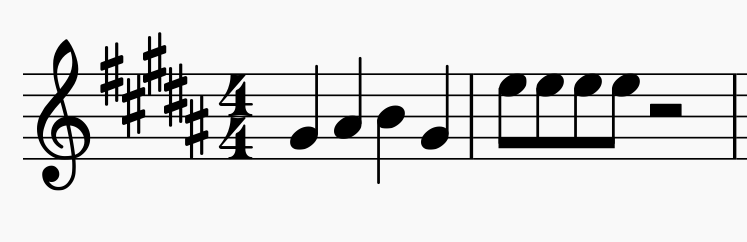
\includegraphics[scale=.5]{res/organ-score.png}}
  \centering
  \caption{Анализ фразы органа Ч0}
    \label{F:5-3-p0}
\end{figure}

\begin{figure}
  \centering
  \subfigure[Спектрограмма]{
    \includegraphics[scale=.5]{build/plot_grayscale_spectrogram.png}}\qquad
  \subfigure[Аппроксимация пиков]{
    \includegraphics[scale=.5]{build/test_peaks_detector.png}}\\
  \centering
  \caption{Анализ фразы органа Ч1}
    \label{F:5-3-p1}
\end{figure}

\begin{figure}
  \centering
  \subfigure[Матрицы W, частотные профили]{
    \includegraphics[scale=.5]{build/plot_w_matrix.png}}\qquad
  \subfigure[Матрица H, временные параметры]{
    \includegraphics[scale=.5]{build/plot_h_matrix.png}}
  \centering
  \caption{Анализ фразы органа Ч2}
    \label{F:5-3-p2}
\end{figure}

В данном примере задача заключается в применении алгоритма NMF
к реальному аудио файлу. Для этой цели был выбрана фраза органа длительностью
13 секунд \cite{L:organ.wav}. На рисунке \ref{F:5-3-p0} представлена
партитура для первых 6 секунд.

На изображении \ref{F:5-3-p1} представлена спектрограмма.
Параметры анализа были выбраны следующими
\begin{verbatim}
  FS = info.SampleRate;
  MFH = 6000;
  M = 2048;
  HS = floor(M * 0.25);
  N = 4096;
  MFS = floor(MFH / FS * N);

  TL = 0.0;
  TR = 5.5;
  SL = floor(TL * FS) + 1;
  SR = floor(TR * FS) + 1;

  x = mean(audioread(info.Filename), 2)(SL : SR);
  [y, c] = stft(x, M, HS, N / 2);
  L = size(y, 2);

  sy = y(1 : MFS, :);

  test_peaks_detector(sy, N, FS);

  plot_grayscale_spectrogram(sy);
\end{verbatim}

Предварительный анализ аудио файла в Sonic Visualizer \cite{L:sonic-visualizer}
показал, что достаточно провести анализ в диапозоне ниже 6000 Гц.

В приложении Д приведен исходный код приложения на языке Octave.

На графиках \ref{F:5-3-p2} представлены результаты факторизации спектрограммы.
Для разложения использовались следующие параметры
\begin{verbatim}
  R = 4;

  [W, H] = innernmf(abs(sy), R, 1e-2);

  plot_h_matrix(L, M, HS, FS, TL, R, H);
  plot_w_matrix(FS, N, MFS, R, W);
\end{verbatim}

Для улучшения результата работы алгоритма, необходимо
\begin{enumerate}
  \item Определить локальные пики на спектрограмме
  \item Аппроксимировать их значения используя параболлическую интерполяцию
  \item Выделить устойчивые пикы как функции частоты по времени,
    частота должна отклоняться в пределах некоторого порога
  \item Полученный вид спектрограммы, отдать на вход алгоритма
\end{enumerate}

На рисунке \ref{F:5-3-p2} можно видеть пример аппроксимации пиков
для исходной спектрограммы, выбранный фрейм является проивзольным.

Как видим большое число пиков имеют небольшое значение амплитуды, следовательно
можно применить отсечение по пороговому значению амплитуды. Это позволит
уменшить число ложных пиков, которые не формируют мелодию органа.

Для улучшения распознавания длительности и времени игры нот
нужно комбинировать результат NMF с другими алгоритмами этого рода.

\cleardoublepage

\section{Music Recognizer}

Для лучшего тестирования было разработано веб-приложение, структурная схема
которого представлена на Диаграмме \ref{F:6-sd}.

\begin{figure}[b]
  \centering
  \begin{tikzpicture}[every node/.style=draw]
    \matrix [matrix of nodes, column sep=5mm, row sep=5mm]
    {
      \node[align=center](a) { Микрофон\\ pyaudio}; & \\
      \node[align=center](b) { WAV файл\\ sms-tools}; &
          \node[align=center](d) {Обработка\\ аудио сигнала\\ pitch-estimator.py};
          & \node[align=center](e)
          {Определение\\ фундаментальной частоты\\ Online-STFT.py}; \\
      \node[align=center](c)
          {Удалённый микрофон\\ (NodeJS, WebSockets,\\ WebAudioAPI)};
          & \node[align=center](f) {Генерация аннотации\\ в build/twm.txt};
          & \node[align=center](g) {Запись аудио сигнала\\ в build/output.wav}; \\
    };

    \draw [line width=0.3mm, ->] (a) -- (d);
    \draw [line width=0.3mm, ->] (b) -- (d);
    \draw [line width=0.3mm, ->] (c) -- (d);
    \draw [line width=0.3mm, ->] (d) -- (e);
    \draw [line width=0.3mm, ->] (e) -- (f);
    \draw [line width=0.3mm, ->] (e) -- (g);

  \end{tikzpicture}
  \caption{Структурная диаграмма}
    \label{F:6-sd}
\end{figure}

\subsection{Определение фундаментальной частоты используя \\
процедуру two-way mismatch}

Определение фундаментальной частоты в квазигармонических сигналах
является важной задачей в обработке музыкальных сигналов.
Процедура \textit{two-way mismatch} (TWM) определения $F_0$ -
это компьютерный метод, который опирается на квазигармоничесность,
что позволяет находить $F_0$ на основе кратковременного спектра входного
сигнала.
Найденная $F_0$ выбирается так, что минимизируется расхождение между
измеренными частотными (синусоидальными) компонентами и гармоническими
компонентами сгенерированными на основе текущего кандидата для $F_0$.
Для каждой пробы $F_0$, несовпадения между сгенерированными гармониками
и измеренными частотными компонентами усредняются на фиксированном
подмножестве доступных компонент. Схема взвешивания используется для
снижения чувствительности процедуры к наличию шума или отсутствию
определенных компонент в спетральных данных.

Алгоритм основан на определении синусоидальных компонент с помощью STFT.
После этого для каждого окна определяется множество $F_0$ и как результат
выбирается та, у которой минимальная ошибка.

Процедура использует следующие функции ошибки:
\begin{align}
  Err_{p \to m} &= \sum_{n=1}^N E_\omega (\Delta f_n, f_n, a_n, A_{max}) \\
                &= \sum_{n=1}^N \Delta f_n \times (f_n) ^{-p} +
                       (\frac{a_n}{A_{max}}) \times [q \Delta f_n \times
                       (f_n)^{-p} - r],
\end{align}

где $\Delta f_n$ есть разница между предсказанными и наиближайшеми измеренными
пиками, $f_n, a_n$ есть частота и магнитуда предсказанных пиков,
$A_{max}$ есть максимальная магнитуда среди пиков.

\begin{align}
  Err_{m \to p} &= \sum_{k=1}^K E_\omega (\Delta f_k, f_k, a_k, A_{max}) \\
                &= \sum_{k=1}^K \Delta f_k \times (f_k) ^{-p} +
                       (\frac{a_k}{A_{max}}) \times [q \Delta f_k \times
                       (f_k)^{-p} - r],
\end{align}

где $\Delta f_k$ есть разница между измеренными и наиближайшеми предсказанными
пиками, $f_k, a_k$ есть частота и магнитуда измеренных пиков,
$A_{max}$ есть максимальная магнитуда среди пиков.

\textbf{Суммарная ошибка:} $Err_{total} = Err_{p \to m}/N + \rho Err_{m \to p}/K$.

Maher и Beauchamp предлагают следующие значения для параметров
$p=0.5, q=1.4, r=0.5, \rho=0.33$.


\cleardoublepage

{\large \bf Заключение \\}
\addcontentsline{toc}{section}{Заключение}
  В заключении отметим результаты проделанного труда:
  \begin{enumerate}
    \item Приведены теоретические сведения о музыке
    \item Приведен теоретические сведения из DSP о дискретном
      преобразовании фурье, о сэмплировании цифровых сигналов
    \item Изучена работа о алгоритмах для решения задачи NMF \cite{DDL}.
      Также частично дан перевод основных положений. В некоторых
      местах текст дополнен практическими замечаниями, которые
      возникли у автора курсовой работы при самостоятельеом изучении
      этого материала и его применении на практике
    \item Изучена работа о применении NMF для решения задачи AMT
      в полифоническом случае \cite{PMTPS}. Была разработана
      программа на её основе, которая распознает частоту
      простейшей полифонической синтетической мелодии.
    \item Реализован на практике алгоритм NMF на основе градиентного
      спуска но с мультипликативными правилами перехода
    \item Реализована на практике функции генерации спектрограмм
      в виде столбцов матриц, которое используется в работе алгоритма
      NMF
    \item В приложении приведены исходные коды некоторых программ
      на языке Octave. Исходный текст всей работ доступен в github
      репозитории автора курсовой работы по ссылке \cite{L:course-paper}.
    \item Разработан прототип веб-приложения для автоматической
      транскрипции музыки
    \item Исследованы существующие разработки в сфере автоматической
      транскрипции музыки
    \item Предложены направления дальнейших исследований для построения
      приложения для потоковой обработки аудио сигналов и генерации
      партитуры
  \end{enumerate}

  Стоит отметить, что исходная формулировка задачи, в которой требуется
  распознать монофоническую мелодию, ещё далеко не решена в данной работе
  и требует дальнейших исследований.

\cleardoublepage

\addcontentsline{toc}{section}{\bibname}
\begin{thebibliography}{0}

  %\bibitem{big_dsp_theory} Manolakis D. Applied digital signal
  %  processing: theory and practice, 2011

  %\bibitem{GDPE} Gerhard D., Pitch Extraction and Fundemental Frequency:
  %  History and Current Techniques, Technical Report TR-CS 2003-06, November,
  %  2003

  %\bibitem{GDCMA} Gerhard D., Computer Music Analysis, Techincal Report CMPT
  %  TR 97-13, October 13, 1997

  %\bibitem{WMT} https://en.wikipedia.org/wiki/Transcription\_(music)

  %\bibitem{WMP} https://en.wikipedia.org/wiki/Pitch\_(music)

  \bibitem{DDL} Lee, D. Algorithms for Non-negative Matrix Factorization /
    D. Lee, H. Sebastian, 2000.

  \bibitem{PMTPS} Smaragdis, P. Non-Negative Matrix Factorization /
    P. Smaragdis, J. Brown, 2003.

  %\bibitem{QUUX} http://www.quuxlabs.com/blog/2010/09/matrix-factorization-a-simple-tutorial-and-implementation-in-python/

  %\bibitem{GGMMIL} George Grätzer, More Math Into LATEX, Fifth edition

  %\bibitem{AKSPMAMT} Anssi Klapuri, Signal Processing Methods for the Automatic
  %  Transcription of Music

  %\bibitem{PCTAM} Nicholas J. Higham,
  %   The Princeton Companion to Applied Mathematics

  %\bibitem{OD} The fourth edition of the Octave documentation

  %\bibitem{ASP} https://www.coursera.org/learn/audio-signal-processing

  \bibitem{L:course-paper}
    Github [Электронный ресурс] - Режим доступа :
    https://github.com/nartes/course-work-amt. -
    Дата доступа : 14.02.2017.

  \bibitem{L:organ.wav}
    Freesound [Электронный ресурс] - Режим доступа :
    https://www.freesound.org/people/nartes/sounds/368365/. -
    Дата доступа : 15.02.2017.

  \bibitem{L:sonic-visualizer}
    SonicVisualiser [Электронный ресурс] - Режим доступа :
    http://www.sonicvisualiser.org/. -
    Дата доступа : 21.02.2017.

  \bibitem{L:sms-tools}
    Github [Электронный ресурс] - Режим доступа :
    https://github.com/MTG/sms-tools. -
    Дата доступа : 20.02.2017.

  \bibitem{L:music-recognizer}
    Github [Электронный ресурс] - Режим доступа :
    https://github.com/nartes/music-recognizer. -
    Дата доступа : 21.02.2017.

  \bibitem{RCMJW} Maher, R. Fundamental frequency estimation of musical signals
    using a two-way mismatch procedure / R. Maher, J. Beauchamp, 1993.

  \bibitem{L:daj-ci-boza}
    Freesound [Электронный ресурс] - Режим доступа :
    https://www.freesound.org/people/MarMaryna/sounds/382598/. -
    Дата доступа : 07.02.2017.

  \bibitem{SBETENN}
    Sigtia, S. An End-to-End Neural Network for Polyphonic Piano Music
    Transcription / S. Sigtia, E. Benetos, S. Dixon, 2015.


  \bibitem{KCFGAMT}
    Choi K. Automatic tagging using deep convolutional neural networks /
    K. Choi, G. Fazerkas, M. Sandler, 2016.

  \bibitem{L:auto-music-tagger}
    Github [Электронный ресурс] - Режим доступа :
    https://github.com/keunwoochoi/music-auto\_tagging-keras. -
    Дата доступа : 20.02.2017.

  \bibitem{L:MAPS}
    Telecom Paristech [Электронный ресурс] - Режим доступа :
    http://www.tsi.telecom-paristech.fr/aao/en/2010/07/08/maps-database-a-piano-database-for-multipitch-estimation-and-automatic-transcription-of-music/. -
    Дата доступа : 03.02.2017.

\end{thebibliography}

%\cleardoublepage

%\appendix

%\section*{Приложение A}\label{A:test2.m}
%\listinginput[1]{1}{src/test2.m}

%\section*{Приложение Б}\label{A:nmf.m}
%\listinginput[1]{1}{src/nmf.m}

%\section*{Приложение В}\label{A:getspectrum.m}
%\listinginput[1]{1}{src/getspectrum.m}

%\section*{Приложение Д}\label{A:realaudio_nmf_post.m}
%\listinginput[1]{1}{src/realaudio_nmf_post.m}

\end{document}
% vi: tabstop=2 sw=2 sts=2
